\documentclass[margin=2mm]{standalone}
\usepackage{tikz}
\tikzset{
  hole/.style = {fill = #1, circle, minimum width = 2.5mm, inner sep = 0mm},
  wire/.style = {draw = #1, line width = .5mm},
  label/.style = {rotate = #1, black!50!white, font=\sffamily, anchor = center},
}
\begin{document}
\newcommand{\wire}[6][]{
  \draw[wire=#2] (#3,#4) edge[#1] (#5,#6);
  \node[hole=#2, minimum width=1mm] at (#3,#4){};
  \node[hole=#2, minimum width=1mm] at (#5,#6){};
}

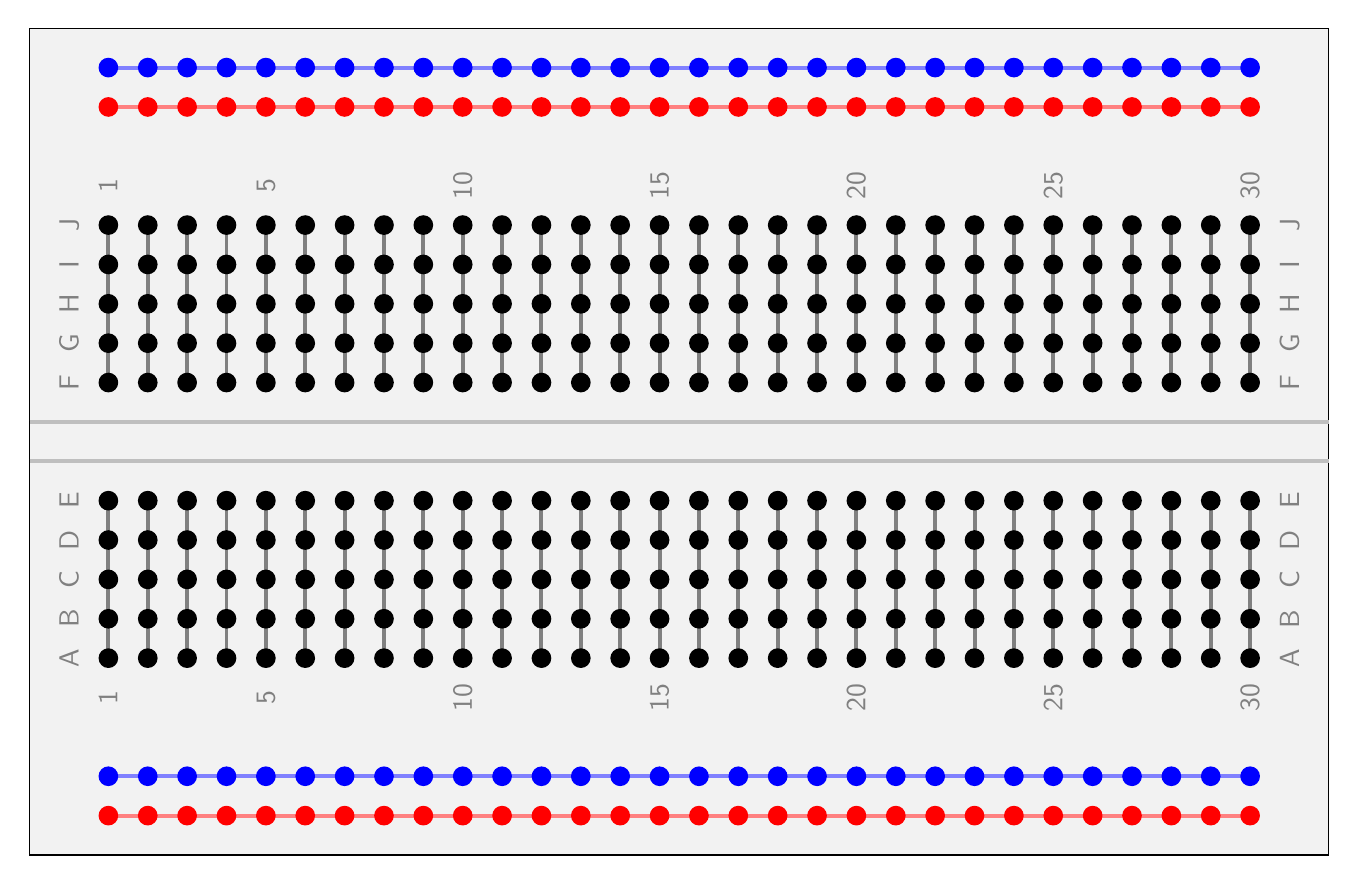
\begin{tikzpicture}[x=5mm,y=5mm]
  \draw[fill=black!05!white] (-1,-4) rectangle (32,17);
  \draw[wire=red!50]  (1,-3) -- (30,-3);
  \draw[wire=blue!50] (1,-2) -- (30,-2);
  \draw[wire=red!50]  (1,15) -- (30,15);
  \draw[wire=blue!50] (1,16) -- (30,16);
  \draw[wire=gray!50] (-1,6) -- (32,6);
  \draw[wire=gray!50] (-1,7) -- (32,7);
  \foreach \xi in {1,...,30}{
    \node[hole=red]  at (\xi,-3){};
    \node[hole=blue] at (\xi,-2){};
    \node[hole=red]  at (\xi,15){};
    \node[hole=blue] at (\xi,16){};
    \foreach \ys in {0,7}{
      \draw[wire=gray] (\xi,1+\ys) -- (\xi,5+\ys);
      \foreach \yi in {1,2,3,4,5}{
        \node[hole=black] at (\xi,\yi+\ys){};
      }
    }
  }
  \foreach \m/\yi in {A/1,B/2,C/3,D/4,E/5,F/8,G/9,H/10,I/11,J/12}{
    \node[label=90] at ( 0,\yi) {\m};
    \node[label=90] at (31,\yi) {\m};
  }
  \foreach \m/\xi in {1,5,10,...,30}{
    \node[label=90] at (\xi, 0) {\m};
    \node[label=90] at (\xi,13) {\m};
  }
\end{tikzpicture}
\end{document}